\chapter{Shogoki: Deterministic Execution} \label{chap:detexec}
A deterministic system provides a property that given the same input, a multithreaded program can always generate the same output. Such a system fits perfectly for our replication purpose. As long as the primary and secondary receive the same input, the replicated application will sure end up with the same state and generate the same output.

For multi-threaded programs, an observation is that as long as the threads don't communicate with each other, the execution is sure to be deterministic\cite{devietti2009dmp}. For example, in pthread based programs, all the inter-thread communications are synchronized by pthread primitives. By making the interleaving of sychronization primitives to be deterministic, the entire program is sure to be deterministic. With this observation, some runtime deterministic solutions actually enforce determinism by trapping pthread primitives\cite{cui2013parrot}\cite{liu2011dthreads}\cite{olszewski2009kendo}. This type of deterministic system is called "Weak Deterministic System". It assumes that the applications are data race free, and only guarantee the deterministic interleaving of thread synchronization primitives such as mutex locks and condition variables. Our implementation falls into this category.

In this chapter we present our Shogoki\footnote{Unit 01}: Deterministic Execution. This replication mode maintains a global execution order, according to this order, an execution token is passed among all the tasks deterministically. Only the task with the execution token can enter the deterministic area, and the token will be held on this task only if it leaves its deterministic area.

%This chapter is structured as follows:
%\begin{itemize}
%\item Section \ref{sec:detsched} shows the basic algorithm and programming interface of the deterministic system.
%\item Section \ref{sec:logimbalance} explains the logical time imbalance problem of this algorithm and two solutions for two different cases.
%\end{itemize}

\section{Logical Time Based Deterministic Scheduling} \label{sec:detsched}
Inspired by Kendo~\cite{olszewski2009kendo} and Conversion~\cite{merrifieldincreasing}, this scheduling policy maintains a logical time for each task inside the current Popcorn namespace. There is a "token" being passed among all the tasks in the namespace according to the logical time of each task. Our system provides following system calls for the applications to control the thread-interleaving:
\begin{itemize}
   \item \_\_det\_start: When it is called, only the task holds the token can proceed. If the current thread is able to proceed, this thread will be marked as "in a deterministic section".
   \item \_\_det\_end: When it is called, the system will increase the current thread's logical time by 1, and marks it as "out of a deterministic section".
\end{itemize}.

The token is updated whenever the logical time is changed, and it is passed based on following rules:
\begin{itemize}
   \item Among all the tasks inside the namespace, the one with the minimal logical time gets the token.
   \item If multiple tasks have the same minimal logical time, the one with the smallest PID gets the token.
\end{itemize}.

\begin{figure}
\centering
\begin{lstlisting}[numbers=left, frame=single, basicstyle=\small, breaklines]{blah}

void producer() {
    while (running){
        item = generate_item();
        syscall(__NR_det_start);
        pthread_mutex_lock(mutex);
        syscall(__NR_det_end);    
        putItem(queue, item);    
        pthread_mutex_unlock(mutex);
    }
}

void consumer() {
    while (running){
        syscall(__NR_det_start);
        pthread_mutex_lock(mutex);
        syscall(__NR_det_end);
        item = getItem(queue);    
        pthread_mutex_unlock(mutex);		
        consume_item(item);
    }
}
\end{lstlisting}
\caption{An example use of the deterministic syscalls}
\label{fig:example}
\end{figure}
Figure~\ref{fig:example} shows an example use of the system calls. Simply wrap pthread\_mutex\_lock with \_\_det\_start and \_\_det\_end will make the acquisition of the mutex to be deterministic.

If the logical time is updated but the one has the minimal logical time is sleeping in \_\_det\_start, the one whose updates the tick will wake the sleeping one up. As long as the replicated application updates logical time in a same way on both primary and secondary, they will sure end up with the same thread interleaving. Figure~\ref{f:algorithm} shows a simplified version of this algorithm (some mutual exclusion points are omitted here).

To make an application to run in a deterministic way, one should put \_\_det\_start and \_\_det\_end around the synchronization primitives such as pthread\_mutex\_lock , so that the order of getting into critical sections is controlled under our deterministic scheduling.

\begin{figure}
\begin{lstlisting}[numbers=left, frame=single, basicstyle=\small, breaklines]{detsys}
void __det_start()
{
    if (token->token != current)
        sleep(current);
    current->ft_det_state = FT_DET_ACTIVE;        
}
void __det_end()
{
    current->ft_det_state = FT_DET_INACTIVE;
    __update_tick(1);
}
void __det_tick(int tick)
{
    __update_tick(tick);
}
void __update_tick(int tick)
{
    current->tick += tick;
    token->task = find_task_with_min_tick(ns);
    if (is_waiting_for_toUponken(token->task))
    	wake_up(token->task);
}
\end{lstlisting}
\caption{Simplified implementation of deterministic system calls}
\label{f:algorithm}
\end{figure}


\subsection{Eliminate Deadlocks} \label{sec:edeadlock}
% cite futex and glic here
With wrapping all the pthread\_mutex\_lock with our deterministic system calls, there is a potential risk of having deadlocks. Serializing all the lock acquisitions with our implementation basically means putting a giant global mutex lock around every lock acquisition. As shown in Figure~\ref{fig:deadlock}, Thread 2 has a lower logical time and try to acquire the mutex(b), however mutex(b) is contended, as a result Thread 2 will call futex\_wait and put the thread into sleep until mutex(b) is released by someone else. At this point, Thread 2 will never increase its logical time until mutex(b) is released. So Thread 1 will never goes through the \_\_det\_start, and it will never unlock mutex(b), which means Thread 2 will never be woken up.

Since we already know that a contented mutex will call futex\_wait~\cite{drepper2005futexes} to wait for a unlock event, the solution to this deadlock problem is to temporary remove the thread in futex\_wait out of the deterministic schedule, and add it back when it returns from futex\_wait. In the example of Figure~\ref{fig:deadlock}, Thread 1 will be able to proceed its \_\_det\_start and keep executing. In order to not to break the determinism, we guarantee the following:
\begin{itemize}
\item We guarantee that the waiting queue in futex\_wait is strictly FIFO, which means the wakeup sequence will be the same as the sequence of getting into futex\_wait. Since the latter one is ensured by our \_\_det\_start, with this hack to futex, the wake up sequence from futex\_wait will be the same sequence determined by previous \_\_det\_start. This is implemented by fixing the priority of each futex object, so that the priority queue inside futex\_wait can behave like a FIFO queue.
\item We guarantee that when waking up from a futex\_wait, the thread always waits for the token before returning to the user space. With this implemented, the timing (in terms of logical time) of getting out of a contended pthread\_mutex\_lock will be deterministic. This is implemented by adding a \_\_det\_start after the wake up point of futex\_wait.
\end{itemize}

\begin{figure}
\centering
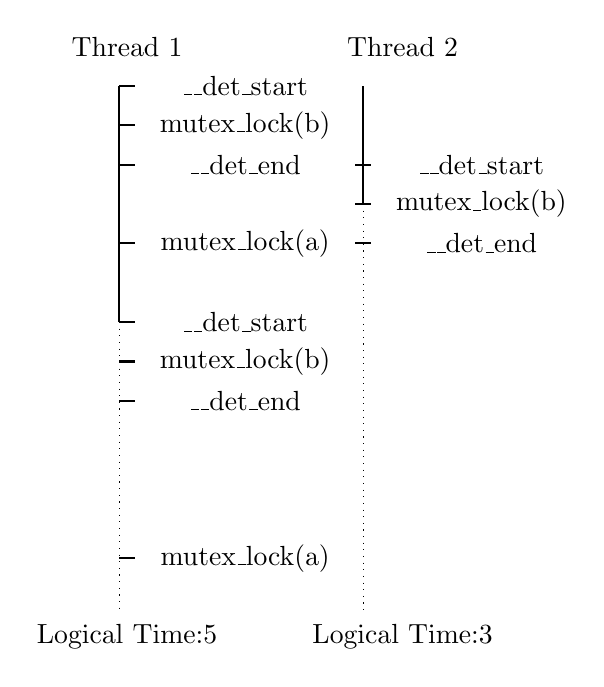
\begin{tikzpicture}
   \draw[thick] (-0.1,4) --  (-0.1,7); 
   \draw[dotted] (-0.1,4) --  (-0.1,0.3);
   
   \node[align=right] at (0,7.5) {Thread 1};
   
   \node[align=right] at (1.5,7) {\_\_det\_start};
   \draw[thick] (-0.1,7) -- (0.1,7);
   \node[align=right] at (1.5,6.5) {mutex\_lock(b)};
   \draw[thick] (-0.1,6.5) -- (0.1,6.5);
   \node[align=right] at (1.5,6) {\_\_det\_end};
   \draw[thick] (-0.1,6) -- (0.1,6);
   \node[align=right] at (1.5,5) {mutex\_lock(a)};
   \draw[thick] (-0.1,5) -- (0.1,5);      
   
   \node[align=right] at (1.5,4) {\_\_det\_start};
   \draw[thick] (-0.1,4) -- (0.1,4);
   \node[align=right] at (1.5,3.5) {mutex\_lock(b)};
   \draw[thick] (-0.1,3.5) -- (0.1,3.5);
   \node[align=right] at (1.5,3) {\_\_det\_end};
   \draw[thick] (-0.1,3) -- (0.1,3);
   \node[align=right] at (1.5,1) {mutex\_lock(a)};
   \draw[thick] (-0.1,1) -- (0.1,1);   
   \node[align=right] at (0,0) {Logical Time:5};
      %show thread 1 holds the lock previously

   \draw[thick] (3,5.5) --  (3,7); 
   \draw[dotted] (3,5.5) --  (3,0.3);
   
   \node[align=right] at (3.5,7.5) {Thread 2};
   \node[align=right] at (4.5,6) {\_\_det\_start};
   \draw[thick] (2.9,6) -- (3.1,6);
   \node[align=right] at (4.5,5.5) {mutex\_lock(b)};
   \draw[thick] (2.9,5.5) -- (3.1,5.5);
   \node[align=right] at (4.5,5) {\_\_det\_end}; 
   \draw[thick] (2.9,5) -- (3.1,5);   
   \node[align=right] at (3.5,0) {Logical Time:3};
\end{tikzpicture}
\caption{An example of deadlock}
\label{fig:deadlock}
\end{figure}

\section{Balance the Logical Time} \label{sec:logimbalance}
Only increasing the logical time by 1 at \detend\ isn't enough. With an example we show how this could break the scalability and how to mitigate this problem. In Figure~\ref{fig:imbalance}, we show a particular execution point of the producer-consumer model in the program snippet we presented in Figure~\ref{fig:example}, solid lines represents the path that is already executed. In this case, consumer reaches consumeItem with logical time 3 and has the token. Assume the real execution time of consumeItem is 10s, which means that when the consumer reaches \_\_det\_end, it would be at least 10s later, that is, the producer has to wait at \_\_det\_start for at least 10s. However we've already enforces the access order of the mutex, the execution out of the critical section should go in parallel since threads don't communicate at that point, in worst case, this kind of waiting will turn a parallel program into a serial program. Figure~\ref{f:pbzip_bad} shows an extreme example where pbzip2 becomes a serial program with unbalanced logical time, it doesn't scale at all as we increase the thread count.

\begin{figure}
\centering
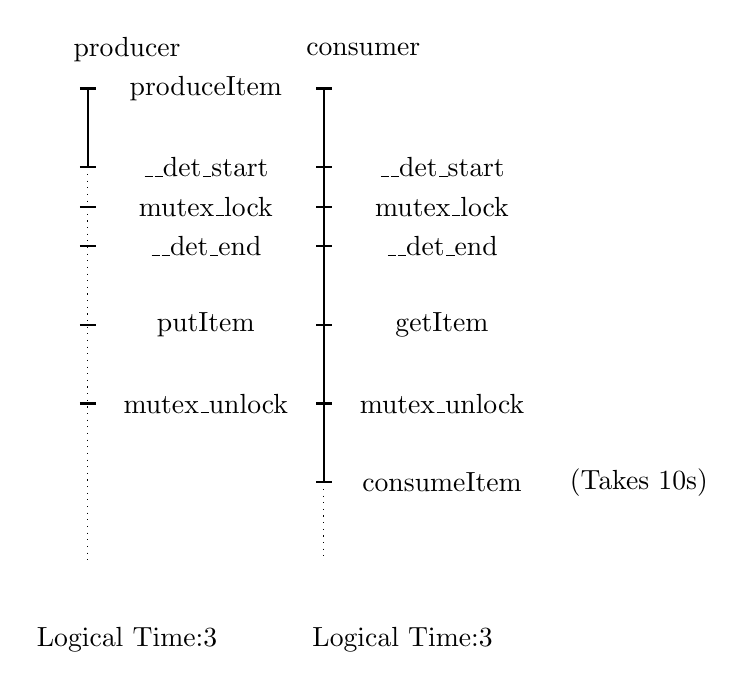
\begin{tikzpicture}
   \draw[thick] (0,4) --  (0,5); 
   \draw[dotted] (0,4) --  (0,-1);
   
   \node[align=right] at (0.5,5.5) {producer};
   \node[align=right] at (1.5,5) {produceItem};
   \draw[thick] (-0.1,5) -- (0.1,5);
   \node[align=right] at (1.5,4) {\_\_det\_start};
   \draw[thick] (-0.1,4) -- (0.1,4);
   \node[align=right] at (1.5,3.5) {mutex\_lock};
   \draw[thick] (-0.1,3.5) -- (0.1,3.5);
   \node[align=right] at (1.5,3) {\_\_det\_end};
   \draw[thick] (-0.1,3) -- (0.1,3);
   \node[align=right] at (1.5,2) {putItem};
   \draw[thick] (-0.1,2) -- (0.1,2);
   \node[align=right] at (1.5,1) {mutex\_unlock};
   \draw[thick] (-0.1,1) -- (0.1,1);   
   \node[align=right] at (0.5,-2) {Logical Time:3};
   
   \draw[thick] (3,0) --  (3,5); 
   \draw[dotted] (3,0) --  (3,-1);
   
   \node[align=right] at (3.5,5.5) {consumer};
   \node[align=right] at (4,5) {};
   \draw[thick] (2.9,5) -- (3.1,5);
   \node[align=right] at (4.5,4) {\_\_det\_start};
   \draw[thick] (2.9,4) -- (3.1,4);
   \node[align=right] at (4.5,3.5) {mutex\_lock};
   \draw[thick] (2.9,3.5) -- (3.1,3.5);
   \node[align=right] at (4.5,3) {\_\_det\_end};
   \draw[thick] (2.9,3) -- (3.1,3);
   \node[align=right] at (4.5,2) {getItem};
   \draw[thick] (2.9,2) -- (3.1,2);
   \node[align=right] at (4.5,1) {mutex\_unlock};
   \draw[thick] (2.9,1) -- (3.1,1);
   \node[align=right] at (4.5,0) {consumeItem};   \node[align=right] at (7,0) {(Takes 10s)};
   \draw[thick] (2.9,0) -- (3.1,0);
   \node[align=right] at (4,-2) {Logical Time:3};   
\end{tikzpicture}
\caption{An example of logical time imbalance.}
\label{fig:imbalance}
\end{figure}

\begin{figure}
\centering
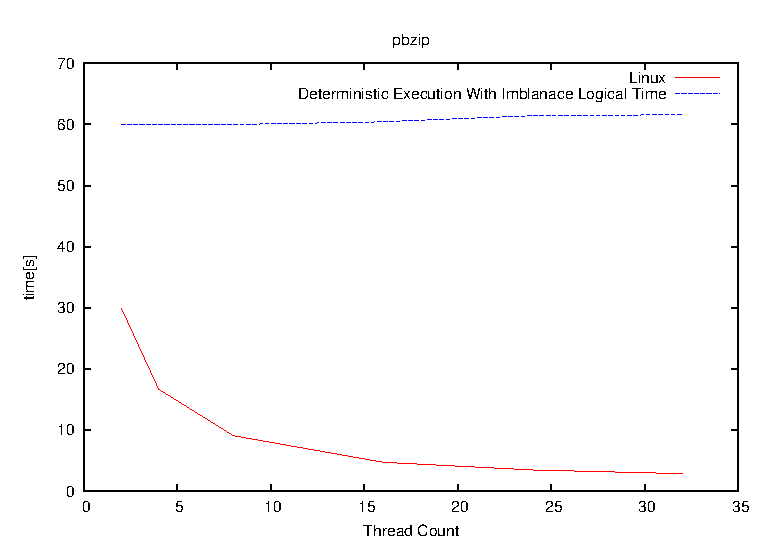
\includegraphics[width=0.8\columnwidth]{figures/pbzip-no-tick}
\caption{pbzip2 without logical time balancing}
\label{f:pbzip_bad}
\end{figure}

Generally, logical time imbalance can happen in two cases:
\begin{itemize}
  \item A task is running for a long time (in user space).
  \item A task is sleeping for a long time (in kernel space).
\end{itemize}

In the upcoming sections we will discuss the solution of each of the cases.
\subsection{Execution Time Profiling}
When a task is running in a computational region (in user space) which might take a long time, the logical time of the task should increase along with the execution. In Kendo this is done by counting retired read instructions — using performance counters — to track to progress of a running task and increases its logical time accordingly. However it is hard to ensure that on the primary and the secondary the performance counter can have the same behaviour~\cite{weaver2008can}, as a result we have to find another way to track the progress of a running task.

Instead of deciding the logical time during the runtime, we discovered a way to settle the logical time during the compilation time. The basic idea is to collect the execution time of via a profile run, then compile the application with the data from the profile run. First, we introduce another system call to increase the logical time of a task:

\begin{itemize}
   \item \_\_det\_tick: This system call comes with a parameter of an integer. When it is called, the logical time will be increased by value defined by the parameter.
\end{itemize}

This system call should be inserted in the program where the logical time needs to be increased. In order to automate this instrumentation process, based on LLVM~\cite{lattner2004llvm}, we implemented two compiler passes to do the profiling and instrumentation.

% show a flow of generating things

\paragraph{Profile Pass}
In order to get the execution time of a program, we make a profile pass to collect the execution time at the granularity of basic block. During the compilation time, this compiler pass will assign a unique number to each basic block, and inserts time profiling functions around every basic block beyond a certain threshold in terms of number of instructions. Figure~\ref{fig:profiled} shows a basic block instrumented with the profile functions in LLVM-IR. In this basic block, bbprof\_start (line 3) and bbprof\_end (line 16) are inserted at the beginning and the end of this basic block.

The profile run is launched by our profile launcher, which will keep track of the execution time of the application, and compute the average execution time for each instrumented basic block upon the application exits. In the end, all the gathered information will be output to a file for future use.

\paragraph{Logical Time Pass}
After the program finished one profile run with the instrumentation of profile pass, we can launch our compiler again to generate the final executable. The logical time pass will take the profile data file as input. This time at the end of each basic block, a \_\_det\_tick will be inserted with the parameter of a scaled execution time of the current basic block. So that the logical time will be bumped at the end of each basic block according to the actual execution time of each basic block. Fi gure~\ref{fig:instrumented} shows an example of instrumented basic block in LLVM-IR. This is the same basic block as we showed in Figure~\ref{fig:profiled}. In this example, Line 9 is the end of the basic block, it comes with a \dettick\ system call with a value 2895535, which is generated and normalized from a previous profile run. In this basic block, line 5 is the most time consuming part in the entire program (pbzip2), as a result this basic block needs a relatively large tick increment.

\begin{figure}
\centering
\begin{lstlisting}[numbers=left, frame=single, basicstyle=\small, breaklines]
if.end.23:                                        ; preds = %for.end
  %38 = load i8*, i8** %CompressedData, align 8
  %39 = call i32 (i32, ...) @bbprof_start(i32 249)
  %40 = load %struct.outBuff*, %struct.outBuff** %fileData, align 8
  %buf = getelementptr inbounds %struct.outBuff, %struct.outBuff* %40, i32 0, i32 0
  %41 = load i8*, i8** %buf, align 8
  %42 = load %struct.outBuff*, %struct.outBuff** %fileData, align 8
  %bufSize24 = getelementptr inbounds %struct.outBuff, %struct.outBuff* %42, i32 0, i32 1
  %43 = load i32, i32* %bufSize24, align 4
  %44 = load i32, i32* @_ZL12BWTblockSize, align 4
  %45 = load i32, i32* @_ZL9Verbosity, align 4
  %call25 = call i32 @BZ2_bzBuffToBuffCompress(i8* %38, i32* %outSize, i8* %41, i32 %43, i32 %44, i32 %45, i32 30)
  store i32 %call25, i32* %ret, align 4
  %46 = load i32, i32* %ret, align 4
  %cmp26 = icmp ne i32 %46, 0
  %47 = call i32 (i32, ...) @bbprof_end(i32 249)
  br i1 %cmp26, label %if.then.27, label %if.end.29
\end{lstlisting}
\caption{An instrumented basic block in pbzip2 with execution time profiling functions.}
\label{fig:profiled}
\end{figure}

\begin{figure}
\centering
\begin{lstlisting}[numbers=left, frame=single, basicstyle=\small, breaklines]
  (.....)
  %bufSize24 = getelementptr inbounds %struct.outBuff, %struct.outBuff* %35, i32 0, i32 1
  %36 = load i32, i32* %bufSize24, align 4
  %37 = load i32, i32* @_ZL12BWTblockSize, align 4
  %38 = load i32, i32* @_ZL9Verbosity, align 4
  %call25 = call i32 @BZ2_bzBuffToBuffCompress(i8* %32, i32* %outSize, i8* %34, i32 %36, i32 %37, i32 %38, i32 30)
  store i32 %call25, i32* %ret, align 4
  %39 = load i32, i32* %ret, align 4
  %cmp26 = icmp ne i32 %39, 0
  %40 = call i32 (...) @syscall(i32 321, i64 2895535)
  br i1 %cmp26, label %if.then.27, label %if.end.29

\end{lstlisting}
\caption{An instrumented basic block in pbzip2 with dettick.}
\label{fig:instrumented}
\end{figure}

\subsection{Tick Bumping for External Events}

When a task is sleeping in the kernel, usually it is in a system call and waiting for some events to wake it up. Especially for system calls like epoll\_wait, poll and accept and other I/O system calls, the arrival time of the event is non-deterministic, as a result, we cannot simply use \dettick\ to increase the logical time with a predefined value from a profile run, because we have no idea how long the thread will be sleeping in the kernel.

Some deterministic systems simply remove the sleeping tasks out of the deterministic schedule and put them back after they are back to user space. This is not applicable in a replication system like ours, as previously stated, the wake up time of those system calls might be different from the primary and secondary replica.
As a result we must not abandon those sleeping tasks, and have to maintain the consistent state of the logical time for those tasks.

% say something about accept, epoll and poll

\begin{figure}
\centering
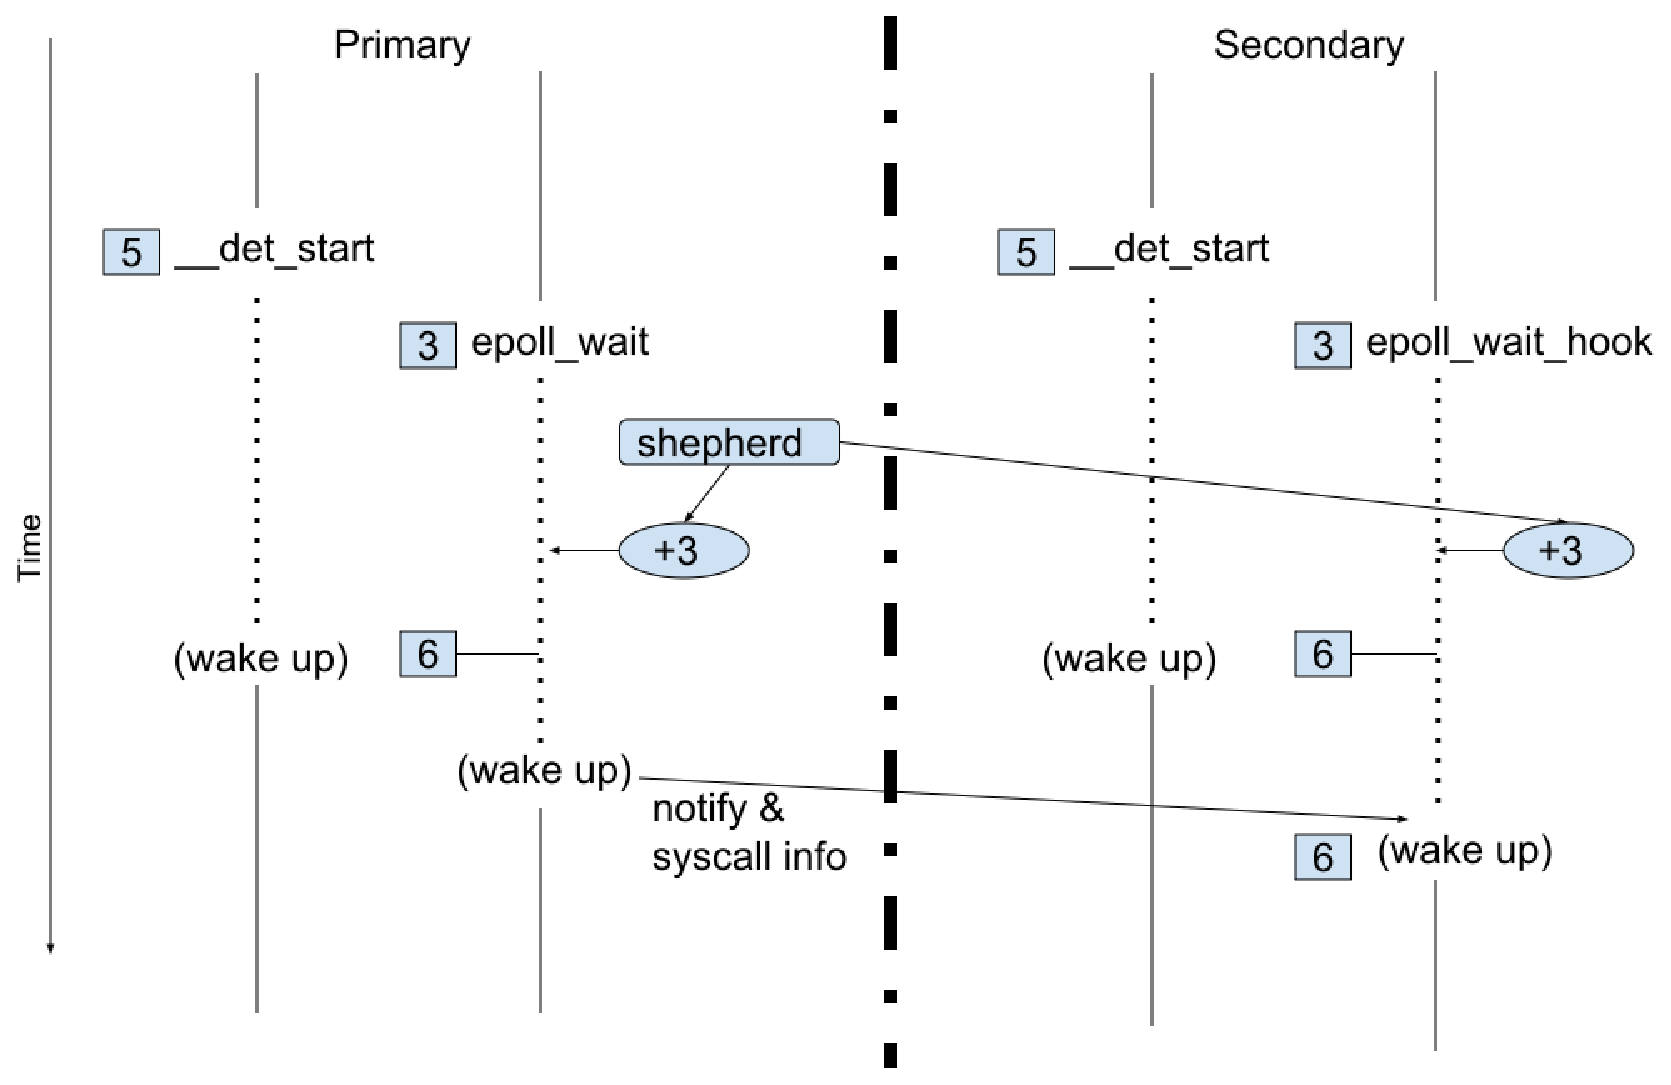
\includegraphics[width=0.8\columnwidth]{figures/tickbump}
\caption{An example of tick bumping}
\label{f:tick_bump}
\end{figure}

In order to let the token passing keep going with those blocking system calls, we need a way to keep bumping those thread's logical time while they are sleeping, a "Tick Shepherd" is implemented to dynamically bump the logical time of the threads that are sleeping in such system calls. The Tick Shepherd is a kernel thread which is mostly sleeping in the background, whenever the token is passed on to a thread that is sleeping on external events or a thread is going to sleep with the token, the shepherd will be woken up to increase the sleeping thread's logical time and send the increased value to the replica. In the meanwhile the corresponding system call on the replica will be blocked at the entry point, and bumps its logical time according to the information from the primary. Figure~\ref{f:tickbump_code} shows the simplified version of Tick Shepherd, it only runs on the primary replica. The syscall on the secondary doesn't proceed until the primary returns from the syscall. In this way we can make sure that when both of the syscalls wake up from sleeping, all the replicas will end up with a consistent state, in terms of logical time. The Tick Shepherd will keep bumping sleeping tasks logical time until for a given period the state of all the tasks comes to a stable point, where nobody makes a single syscall. After that, it will go back to sleep again.

Figure~\ref{f:tick_bump} shows an example of how Tick Shepherd works in action. In this example, tick shepherd detects the token is on a thread sleeping in epoll\_wait, so it bumps its tick by 3 and sends this info to the secondary so that the token can leave this thread. And after the primary returns from epoll\_wait, it sends a message to the secondary, so that the corresponding thread can start to execute its epoll\_wait and uses the output from the primary as its own output. In order to be efficient, we only let Tick Shepherd to bump the system calls that for sure will be called for deterministic times, the current implementation covers all the major I/O related system calls.

\begin{figure}
\begin{lstlisting}[numbers=left, frame=single, basicstyle=\small, breaklines]{tickshepherd}
/*
 * Definitions:
 * ns: current popcorn namespace
 * ns->token: a pointer pointing to the task holds the token
 * current->ft_det_tick: logical time of the task
 * current->ft_pid: replicated task unique identifier
 */
while (!kthread_should_stop()) {
  if (ns->task_count == 0 ||
    ns->wait_count == 0) {
    sleep(); // Sleep until some task wakes it up
    continue;
  }
  token = ns->token;
  tick = token->task->ft_det_tick;
  udelay(20); // delay for a small duration
  token2 = ns->token;
  tick2 = token2->task->ft_det_tick;
  // Which means the token hasn't been changed during the delay,
  // It's time to bump the tick
  if (token == token2 && tick2 == tick) {
    if (!is_waiting_for_token(token->task) &&
      (is_concerned_syscall(token->task->current_syscall)) {
        if (ns->wait_count != 0 &&
          token->task->bumped == 0) {
            bump_task = token->task;
            id_syscall = token->task->id_syscall;
            bump = ns->last_tick + 1;
            previous_bump = token->task->ft_det_tick;
            token->task->ft_det_tick = ns->last_tick + 1;
            update_token(ns);
            send_bump(bump_task, id_syscall, previous_bump, bump);
            continue;
         }
      }
   }
}
\end{lstlisting}
\caption{Simplified implementation of Tick Shepherd}
\label{f:tickbump_code}
\end{figure}

\section{Related Work}
Deterministic execution is the most intuitive way of implementing a state machine replication system. However most of the existing deterministic systems are not suitable for production environments as mentioned in previous discussions ~\cite{bergan2011deterministic}, they are either domain specified, or too slow, or need hardware support. In the following subsections we will discuss the problems in each category of deterministic execution, also the existing solutions for applying deterministic execution to replication.

%In a recent discussion ~\cite{bergan2011deterministic}, it is mentioned that 

\subsection{Deterministic Language Extension}
Clik++~\cite{leiserson2010cilk++} is an parallel extension to C++ which makes creating parallel program easier. This extension provides a property that can indicate threads to be executed in a serial way, so that the determinism can be ensured. Grace \cite{berger2009grace} is also a C++ extension that adds a fork-join parallel schema to C++, it enforces the determinism of the execution with its underlying language runtime. Both of them are very limited to a specific parallel programming model, and existing applications need to be rewritten to achieve determinism.

\subsection{Software Deterministic Runtime}
\subsubsection{Weak Determinism}
Weak Deterministic systems usually only target on making synchronization primitives to be deterministic. Kendo\cite{olszewski2009kendo}, Parrot\cite{cui2013parrot} and Dthreads\cite{liu2011dthreads} are three typical weak deterministic systems, they provide runtime substitutions for pthread library. By making pthread synchronizations to be deterministic, any race-free pthread-based application can be executed in a deterministic way. They are easy to be applied onto existing applications. Our implementation falls in to this category and the basic algorithm derives from Kendo. In order to address the logical time imbalance problem, Kendo relies on hardware counters to keep track of the program's progress in runtime, given the fact that hardware counters could be non-deterministic\cite{weaver2008can}, for our replication use, it might not be worth to put too much engineering efforts to make the performance counters on both kernels to be synchronized.

\subsubsection{Strong Determinism}
Strong Deterministic systems aims to make every shared memory access to happen in a deterministic order. Consequence~\cite{merrifield2015high} and dOS~\cite{bergan2010deterministic} both provide an OS layer to make shared memory access to be deterministic, which is applicable for all kinds of parallel programming models. However their overhead is too high due to massive trapping to shared memory accesses, with this kind of overhead (at least 1X) it is not practical for them to be used in production. DMP~\cite{devietti2009dmp} based on dOS, introduces hardware transaction memory to accelerate the memory trapping process. In our replication use case, such strong determinism is not needed, as we only need need the output of replicated applications to be the same. The effort for enforcing strong determinism would put too much unnecessary overhead.

\subsection{Architectural Determinism}
In ~\cite{segulja2012architectural} and ~\cite{hower2011calvin}, the authors both proposed architectural solutions to ensure memory access determinism. The goal for such systems is to track all the memory access and does versioning on the memory operations. By doing deterministic submission to the memory hierarchy, they are able to ensure the determinism of the parallel execution. RCDC~\cite{devietti2011rcdc} proposes a software/hardware hybrid solution to provide a relaxed deterministic access to the shared memory regions. All are promising solutions to provide a transparent deterministic execution environment, but those designated hardware support cannot be easily satisfied on commodity hardware. 

\subsection{Deterministic System For Replication}
Almost all the deterministic systems mentioned the use case for replication but few provides an actually solution. Theoretically, all the deterministic systems mentioned so far are able to be applied for replication, but only for applications that do not have any network communication. The major challenge for replicating concurrent network applications is the arrival time of the network events is non-deterministic and unpredictable. In order to make the replicas be consistent, the replicas have to process the requests on the same state. All the weak deterministic systems mentioned so far either did not mention network operations(Dthreads\cite{liu2011dthreads}) or simply skip the threads doing such operations (Kendo\cite{olszewski2009kendo}, Parrot\cite{cui2013parrot}), leave them out of the deterministic scheduling.

Actually skipping the threads sleeping in network events is applicable with some workarounds, as long as the system can ensure that when those threads are back from sleeping, all the replicas can be in the same state. A solution is to delay the wakeup time of those threads a little bit until all the replicas reach the same state. We investigated the skipping strategy with Kendo's algorithm, a possible solution is to bump the logical time of the sleeping threads to a relatively high value, so that when they are back to the deterministic schedule, no running thread can have a higher logical time other then them. We modelled such strategy with a multi-threaded network server in TLA+ and proved the correctness of it. However, in practical, it is very hard to pre-determine such a future logical time for the unpredictable network events, furthermore, delaying the wakeup time of those threads will sure have impact on the performance. As a result, we chose to not to skip any socket operations and ended up with the current Tick Shepherd solution.

Several works showed the same idea that network operations should not be skipped, dOS~\cite{bergan2010deterministic} mentioned a use case for replicating a micro web server, which uses the SHIM layer to block the network requests until the all replicas reach the same state. This solution will harm the performance badly and requires modifications to the application. Crane~\cite{cui2015p} utilizes Parrot\cite{cui2013parrot} as the underlying deterministic system but without skipping the network operations. On top of that, Crane uses Paxos to bridge the gap between non-deterministic socket requests and the deterministic system, which ensures that all the replicas can receive the requests in the same state. However, Crane does not show any performance scalability in their work, and with our experiment on Crane, their Paxos layer becomes very unstable with large number of network requests.